\subsubsection{Polarized PDFs}
\label{sec:polPDFs}

Like their unpolarised (spin-averaged) counterparts described in the previous 
subsection, helicity PDFs, along with estimates of their uncertainties, can be 
determined from a comprehensive global analysis of the available spin-dependent 
data. 
%
Here we delineate the aspects of the framework specific to the polarised
case, and give a brief review of current global polarised PDF fits.

\paragraph{General framework.}
%
%
The dependence on the momentum fraction $x$, fixed by non-perturbative QCD 
dynamics, should satisfy some theoretical constraints.
%
First, PDFs must lead to positive cross sections.
At leading order (LO), this implies that polarised 
PDFs are bounded by their unpolarised counterparts\footnote{Beyond LO, more 
complicate relations hold~\cite{Altarelli:1998gn}; however they have little
effect on PDFs.}, $|\Delta f(x,\mu^2)|\leq f(x,\mu^2)$.
%
Second, PDFs must be integrable: this corresponds to the assumption 
that the nucleon matrix element of the axial current for each flavour is finite.
%
Third, SU(2) and SU(3) flavour symmetry, if assumed to be exact, imply that 
the first moments of the nonsinglet $\mathcal{C}$-even PDF combinations,
$\Delta T_3=\Delta u^+ -\Delta d^+$ and 
$\Delta T_8 = \Delta u^+ +\Delta d^+ -2\Delta s^+$ 
(where $\Delta q^+=\Delta q+\Delta\bar{q}$, $q=u,d,s$), are respectively
related to the baryon octet $\beta$-decay constants, whose 
measured values values are~\cite{Olive:2016xmw}
\begin{align}
 a_3
 & =
 \int_0^1 dx \Delta T_3 (x,\mu^2)
 = \langle 1\rangle_{\Delta u^+} - \langle 1\rangle_{\Delta d^+}  = 1.2701 \pm 0.0025\\
 a_8
 & =
 \int_0^1 dx \Delta T_8 (x,\mu^2)
 = \langle 1 \rangle_{\Delta u^+} + \langle 1 \rangle_{\Delta d^+} -2\,\langle 1 \rangle_{\Delta s^+} 
 =0.585  \pm 0.025
 \,\mbox{.}
\label{eq:decayconst}
\end{align}
%
Fairly significant violations of SU(3) symmetry are advocated
in the literature (see {\it e.g.} Ref.~\cite{Cabibbo:2003cu} for a review). 
%
In this case, an uncertainty on the octet axial charge, larger by up to $30\%$ 
than its experimental value in Eq.~\eqref{eq:decayconst}, 
is found~\cite{FloresMendieta:1998ii}. 

The bulk of the experimental information on polarised PDFs comes from 
neutral-current (photon exchange) inclusive and semi-inclusive deep-inelastic scattering 
(DIS and SIDIS) with charged lepton beams and nuclear targets. 
%
As the photon scattering does not distinguish quarks and antiquarks, inclusive DIS 
data constrain only the total quark combinations $\Delta q^+$, 
while SIDIS data with identified pions or kaons in the final state 
constrain individual quark and antiquark flavours. 
%
In principle, both DIS and SIDIS are also sensitive to the gluon 
distribution $\Delta g$, as it directly enters the factorised expressions of
the corresponding structure functions beyond LO, and indirectly via DGLAP 
evolution.
%
In practice the constraining power of DIS and SIDIS data on $\Delta g$ is 
rather weak, because of the limited $Q^2$ range covered by the data. 

Note that, in the case of SIDIS, a reliable knowledge of fragmentation 
functions (FFs) is required in the factorised expressions of the 
corresponding observables. 
%
Since FFs are non-perturbative objects on the same footing as PDFs, they are 
an additional source of uncertainty in the PDF determination, and can  
even become a bias.
%
For this reason, a significant experimental and theoretical effort has been
put in improving the independent determination of 
FFs~\cite{deFlorian:2014xna,deFlorian:2017lwf,
Hirai:2016loo,Sato:2016tuz,Nocera:2017qgb,Bertone:2017xsf,Ethier:2017zbq}.

Besides DIS and SIDIS fixed-target data, a significant amount of data from
longitudinally polarised proton-proton ($pp$) collisions at the Relativistic 
Heavy Ion Collider (RHIC) have become available recently (see {\it e.g.} 
Ref.~\cite{Aschenauer:2015eha} for an overview), although in a limited range 
of momentum fractions, $0.05\lesssim x \lesssim 0.4$.
%
On the one hand, longitudinal (parity-violating) single-spin and 
(parity-conserving) double-spin asymmetries for $W^\pm$ boson production are 
sensitive to the flavour decomposition of polarised quark and antiquark 
distributions, because of the chiral nature of the weak 
interactions~\cite{Bourrely:1993dd}. 
%
On the other hand, double-spin asymmetries for jet, di-jet and $\pi^0$ 
production are directly sensitive to the gluon polarization in 
the proton, because of the dominance of gluon-gluon and quark-gluon initiated 
subprocesses in the kinematic range accessed by RHIC~\cite{Bourrely:1990pz}.

The kinematic coverage of the data which can be used to constrain polarised 
PDFs is displayed in Fig.~\ref{fig:kinEIC}.
%
A comparison with Fig.~\ref{fig:kinplot-report} makes it apparent that the
quantity of data points, their kinematic coverage and the variety of 
available hard-scattering processes are presently much more limited in the polarised case
than in the unpolarised case.
%
Therefore polarised PDFs can currently be determined with much less 
precision than their unpolarised counterparts and also only over an $x$-range limited
to $x\gtrsim 0.005$.
%
The kinematic coverage is expected to be significantly extended in the future,
with DIS and SIDIS data from JLab-12~\cite{Dudek:2012vr} and a polarised 
high-energy Electron-Ion Collider (EIC)~\cite{Accardi:2012qut}.
%
Such an extended kinematic coverage is also displayed in Fig.\ref{fig:kinEIC}.
%
The eRHIC realisation of an EIC~\cite{Aschenauer:2014cki} has been considered.

%-------------------------------------------------------------------------------
\begin{figure}[!t]
\centering
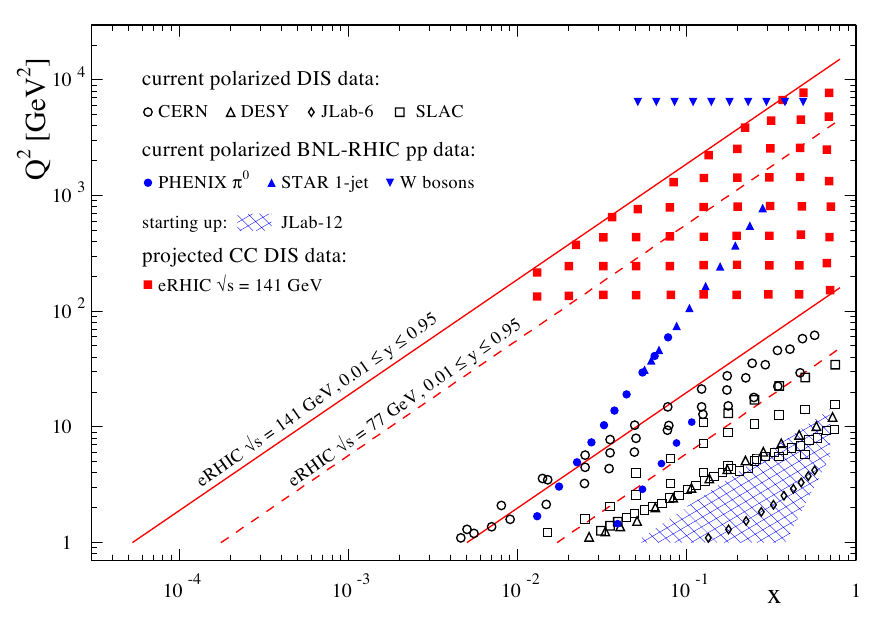
\includegraphics[width=0.9\textwidth]{plots/kinEIC}\\
\caption{\small Representative kinematic coverage, in the $(x,Q^2)$ plane,
of the (neutral current) DIS, SIDIS and $pp$ hard-scattering measurements 
that are used as input in a global polarised PDF fit.
%
The extended kinematic coverage achieved by 
JLab-12~\cite{Dudek:2012vr} and by the eRHIC~\cite{Aschenauer:2014cki} 
realisation of an EIC~\cite{Accardi:2012qut}
(including projected charged-current (CC) DIS data) is also shown.
%
Figure taken from Ref.~\cite{Aschenauer:2014cki}.}
\label{fig:kinEIC}
\end{figure}
%-------------------------------------------------------------------------------

A representative illustration of polarised PDFs obtained from a global
QCD analysis, namely NNDPFpol1.1~\cite{Nocera:2014gqa}, is provided in Fig.~\ref{fig:qPDFpol}.
%
The format is the same as for the unpolarised case, Fig.~\ref{fig:nnlopdfs},
in order to ease any comparison between the two.
%
In particular, note the suppression of all polarised PDFs at small values of 
$x$, including polarised sea quark PDFs, with respect to their unpolarised 
counterparts.

%-------------------------------------------------------------------------------
\begin{figure}[!t]
\centering
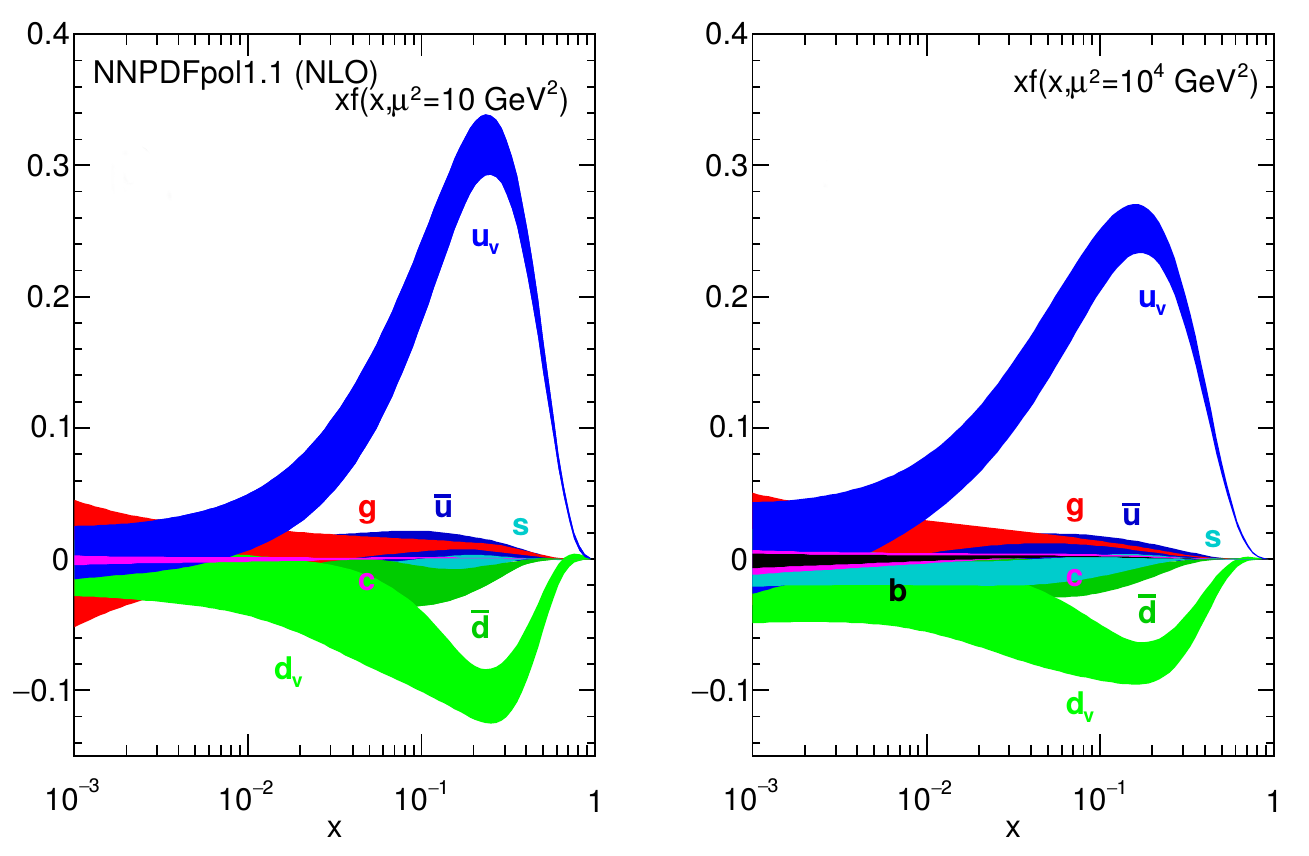
\includegraphics[scale=0.4]{plots/NNPDFpol}\\
\caption{\small Same as Fig.~\ref{fig:nnlopdfs}, 
but for the polarised NNPDFpol1.1 NLO PDFs~\cite{Nocera:2014gqa}.}
\label{fig:qPDFpol}
\end{figure}
%-------------------------------------------------------------------------------

\paragraph{State-of-the-art global polarised PDF fits.}

Several modern determinations of polarised PDFs of the proton (up to 
NLO\footnote{A NNLO QCD analysis of polarised PDFs based on inclusive DIS
data only was performed in Refs.~\cite{Shahri:2016uzl,Khanpour:2017cha}.
Inclusive DIS is the only polarised process for which coefficient functions
are known up to NNLO (all others are known only up to NLO).} 
and mostly in the $\overline{\rm MS}$ factorization scheme) are available in 
the literature~\cite{Nocera:2014gqa,Nocera:2016xhb,deFlorian:2014yva,deFlorian:2008mr,deFlorian:2009vb,Sato:2016tuz,Leader:2010rb,Blumlein:2010rn,Bourrely:2014uha,Hirai:2008aj}. 
%
A key goal of these is to also unveil the size (and uncertainty) of
$\Delta\Sigma$ and  $\Delta G$ in Eq.~\eqref{eq:moments}. 
%
The various determinations differ among each other in the data sets included 
in the analysis, in some details of the QCD analysis (like the treatment of 
higher-twist corrections) and in the procedure used to determine PDFs from the 
data (for details, see {\it e.g.} Chap.~3 in Refs.~\cite{Nocera:2014vla} 
and~\cite{Nocera:2016xhb}). 
%
The NNDPF procedure and the conventional/standard one adopted by DSSV have 
already been outlined in Sec.~\ref{sec:unpPDFs}. 
%
We note that DSSV has developed a method based on Mellin moments of the PDFs 
in order to efficiently incorporate NLO computations
of $pp$ cross sections in the fitting procedure. 
%
The JAM collaboration has implemented for their analysis a new approach called 
iterative Monte Carlo procedure~\cite{Sato:2016tuz}. 

Motivated by the interest in assessing the impact of RHIC $pp$ 
data, two new global analyses of polarised PDFs have been carried out in
2014, DSSV14~\cite{deFlorian:2014yva} and NNPDFpol1.1~\cite{Nocera:2014gqa}.
%
They upgrade the corresponding previous analyses, 
DSSV08~\cite{deFlorian:2008mr,deFlorian:2009vb} and 
NNPDFpol1.0~\cite{Ball:2013lla}, with data respectively on double-spin 
asymmetries for inclusive jet production~\cite{Adamczyk:2014ozi} 
and $\pi^0$ production~\cite{Adare:2014hsq}\footnote{Preliminary RHIC results 
included in Ref.~\cite{deFlorian:2008mr} were replaced in
Ref.~\cite{deFlorian:2014yva} with final results.}, 
and on double-spin asymmetries for high-$p_T$ inclusive jet 
production~\cite{Adamczyk:2014ozi,Adamczyk:2012qj,Adare:2010cc} and single-spin
asymmetries for $W^\pm$ production~\cite{Adamczyk:2014xyw}.
%
The new data have been included in NNPDFpol1.1 
by means of Bayesian reweighting~\cite{Ball:2010gb},
and in DSSV14 by means of a full refit.  

Overall, both the DSSV14 and NNPDFpol1.1 PDF determinations are 
state-of-the-art in the inclusion of the available experimental information. 
%
The data sets in the two analyses differ between each other only in
fixed-target SIDIS and RHIC $\pi^0$ production measurements, included in 
DSSV14, but not in NNPDFpol1.1. 
%
The information brought in by these data is complementary to that provided by 
RHIC $W^\pm$ production and inclusive jet production data respectively,
although fraught with larger theoretical uncertainties related to fragmentation.

%------------------------------------------------------------------------------
\begin{figure}[!t]
%\centering

\hspace*{6mm}
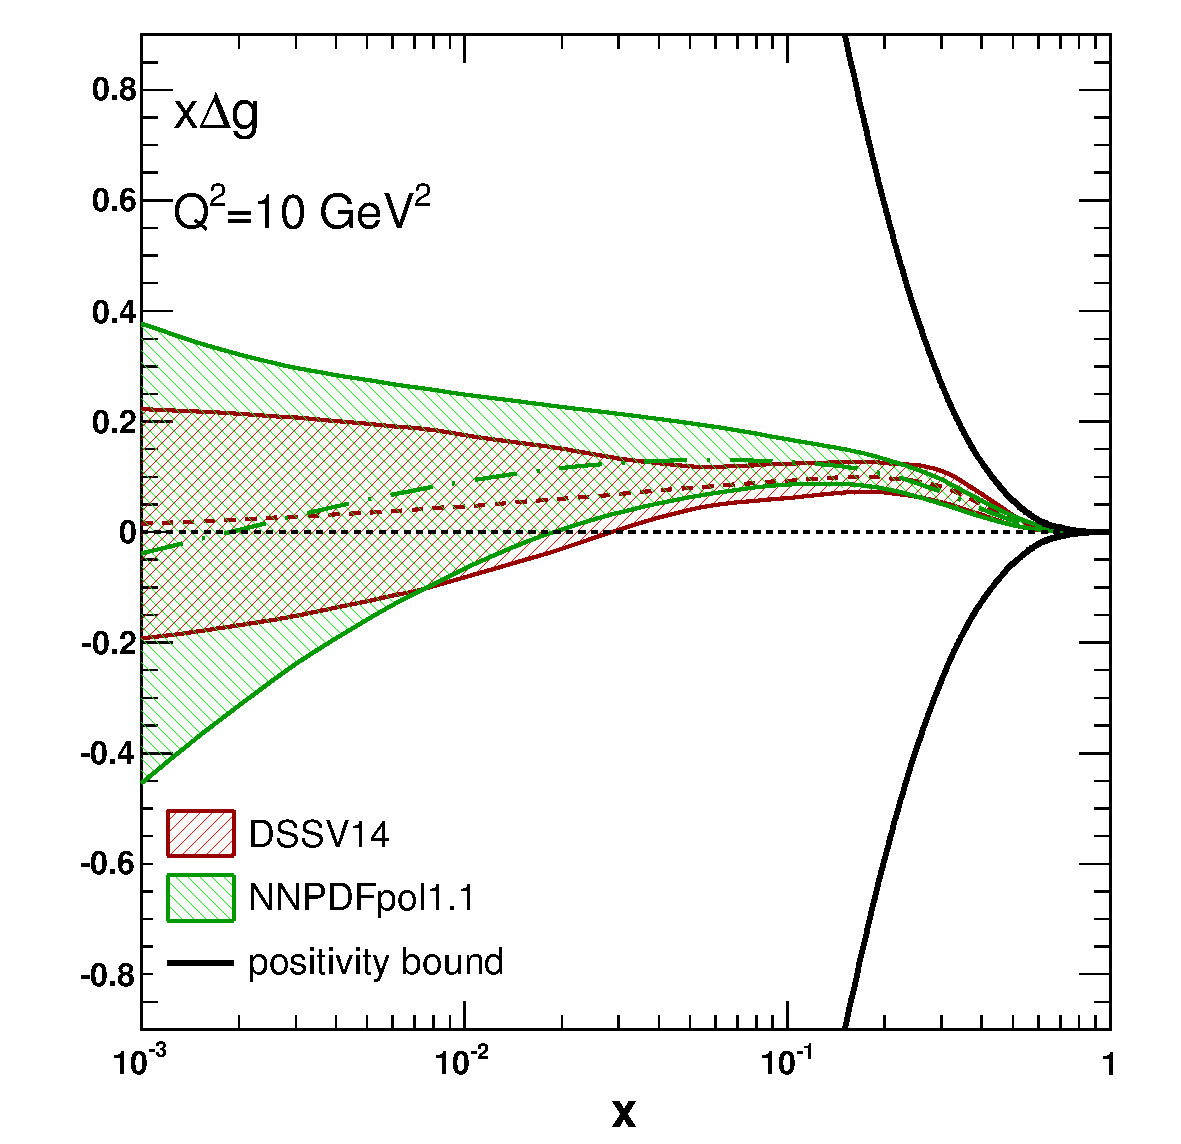
\includegraphics[scale=0.325]{plots/gluoncomp}

\vspace*{-15.1cm}
\hspace*{8cm}
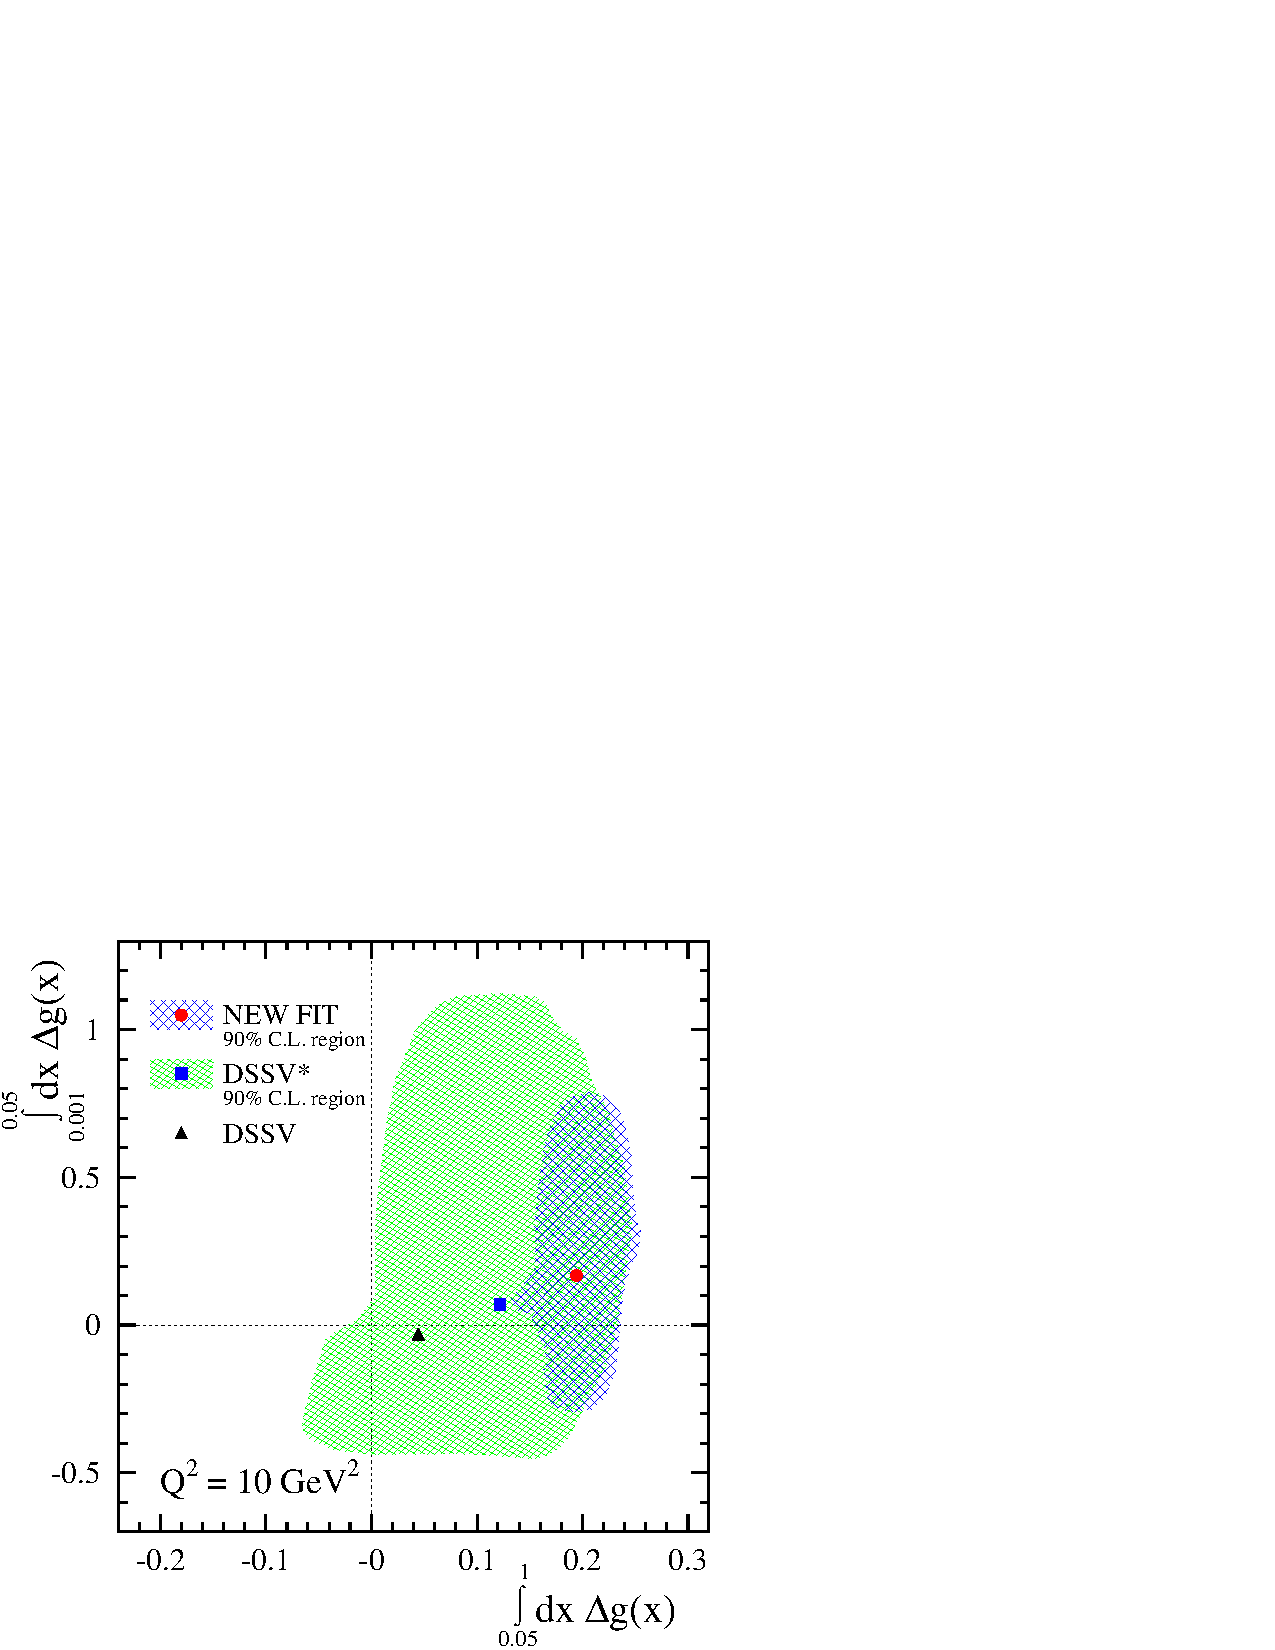
\includegraphics[scale=0.555]{plots/correlation_getot.pdf}

\caption{(Left) The polarised gluon momentum distribution  $x\Delta g$ from the 
DSSV14 (with $90\%$ C.L. uncertainty band)
and NNPDFpol1.1 PDF sets at $Q^2=10$ GeV$^2$. The NNPDF3.1 positivity
bound is also shown.
(Right) $90\%$ C.L.\ areas in the plane spanned by the truncated moments of
$\Delta g$ computed for $0.05\leq x\leq 1$ and $0.001\leq x\leq 0.05$ at $Q^2=10\,\mathrm{GeV}^2$~\cite{deFlorian:2014yva}.}
\label{fig:RHICpdfs}
\end{figure}
%------------------------------------------------------------------------------

The effect of RHIC data on the polarised PDFs of the proton is twofold:
\begin{itemize}

\item The 2009 STAR and PHENIX data sets on jet and $\pi^0$ 
production~\cite{Adamczyk:2014ozi,Adare:2014hsq}, included in DSSV14
and NNPDFpol1.1, provide the first evidence
of a sizable positive gluon polarization in the proton. 
%
A comparison of the gluon PDF in the two PDF sets is displayed in 
Fig.~\ref{fig:RHICpdfs} (left panel). 
%
Comparable results, both central values and uncertainties, are found in the 
$x$ region covered by RHIC data. 
%
The agreement between the two analyses is optimal in the
range $0.08\leq x \leq 0.2$, where the dominant experimental information comes
from jet data; a slightly smaller central value is found in the DSSV14 
analysis, in comparison to the NNPDFpol1.1, in the range 
$0.05\leq x \leq 0.08$, where the dominant experimental information comes from 
$\pi^0$ production data. 
%
Indeed, these are included in DSSV14 but are not
in NNPDFpol1.1. 
%
Nevertheless, best fits lie well within each other error
bands, though NNPDFpol1.1 uncertainties tend to be larger than DSSV14
uncertainties outside the region covered by RHIC data.
%
Very well consistent values of the integral of $\Delta g$, 
Eq.~\eqref{eq:moments}, truncated over the interval $0.05\leq x \leq 1$, are 
found: at $Q^2=10$ GeV$^2$, this is $0.20^{+0.06}_{-0.07}$ for 
DSSV14~\cite{deFlorian:2014yva}, and $0.23\pm 0.06$ for 
NNPDFpol1.1~\cite{Nocera:2014gqa}. The right plot in Fig.~\ref{fig:RHICpdfs} 
shows the corresponding DSSV14 result as an example; the impact of the RHIC
data is clearly visible. 

\item The 2012 STAR data sets on $W$ production~\cite{Adamczyk:2014xyw}, 
included in NNPDFpol1.1, provide evidence of a positive 
$\Delta\bar{u}$ distribution 
and a negative $\Delta\bar{d}$ distribution, with 
$|\Delta\bar{d}|>|\Delta\bar{u}|$~\cite{Nocera:2014gqa},
as shown in Fig.~\ref{fig:RHICpdfs1}.
% 
The size of the flavour symmetry breaking for polarised sea quarks is 
quantified by the asymmetry $\Delta\bar{u}-\Delta\bar{d}$, which,
in the NNPDFpol1.1 analysis, turned out to be roughly as large as its 
unpolarised counterpart (in absolute value), 
though much more uncertain~\cite{Nocera:2014rea}. 
%
Even within this uncertainty, polarised and unpolarised light sea quark 
asymmetries show opposite signs,
with the polarised ones being clearly positive.  This trend is also found
from analysis of the polarized SIDIS data, as revealed by the DSSV analyses. 
%
This result may discriminate among models of nucleon structure; 
see Fig.~\ref{fig:RHICpdfs1}: 
specifically, some meson-cloud (MC) models are disfavored, while a more 
accurate experimental information is needed to establish whether 
chiral quark-soliton (CQS), Pauli-blocking (PB) or statistical (ST)
models are preferred (all these models are described in 
Ref.~\cite{Chang:2014jba}).

\end{itemize}

%------------------------------------------------------------------------------
\begin{figure}[!h]
\centering
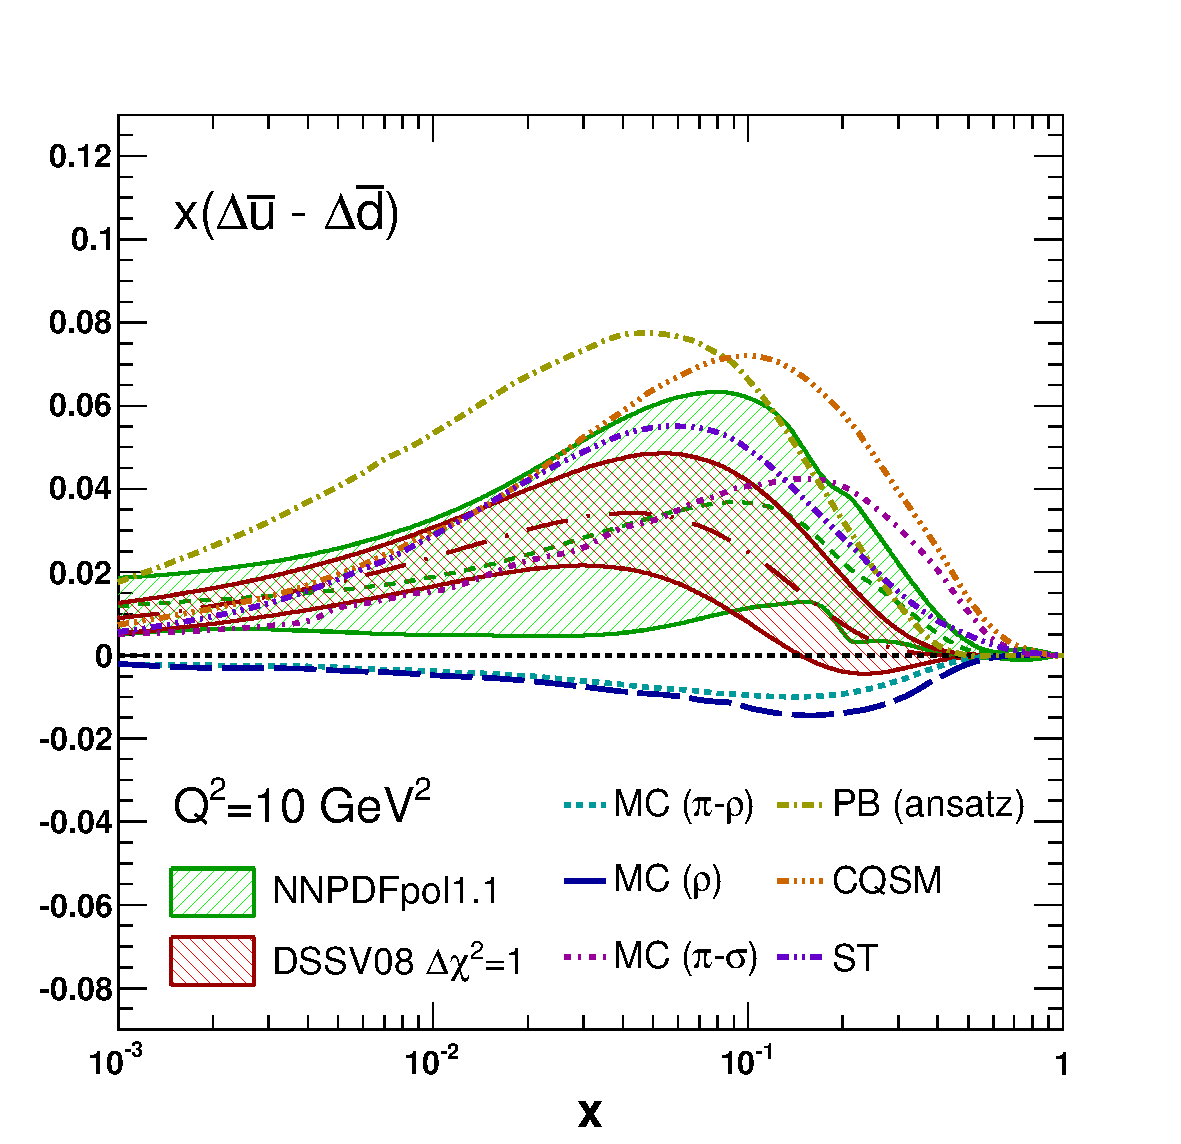
\includegraphics[scale=0.35]{plots/asysea_2}\\
\caption{The polarised light sea quark asymmetry 
$x(\Delta\bar{u}-\Delta\bar{d})$ from the NNPDFpol1.1 and 
DSSV08 PDF sets at $Q^2=10$ GeV$^2$, compared to expectations from 
various models of nucleon structure~\cite{Chang:2014jba}.}
\label{fig:RHICpdfs1}
\end{figure}
%------------------------------------------------------------------------------
\paragraph{Open issues.}

Despite the achievements described above, the polarised PDFs presently cannot 
be determined in a global QCD analysis with the same accuracy as their 
unpolarised counterparts.
%
The experimental data are so far confined to a relatively narrow range of 
$x$ and $Q^2$.
%
As a consequence, the sizes of the contribution of quarks, antiquarks and 
gluons to the nucleon spin, as quantified by their first moments, 
Eq.~\eqref{eq:moments}, are still affected by large uncertainties. 
%
These come predominantly from the extrapolation into the small-$x$ region 
($x\lesssim 10^{-3}$). 
%
Here potential modifications in the PDF shape induced by small-$x$ evolution 
could arise, which presently cannot be tested.
%
Significant uncertainties also affect the PDFs in the large-$x$ 
{\it valence} region ($x\gtrsim 0.7$). 
%
This regime is less relevant for determination of the first moments, but is 
important for comparisons to nonperturbative models of nucleon structure, 
especially in terms of ratios of light-quark polarised to unpolarised PDFs 
(for a comparison between large-$x$ PDFs 
and model predictions, see Ref.~\cite{Nocera:2014uea}).
%
Finally, the small lever arm of the data in $Q^2$ is a serious limiting factor 
in the determination of $\Delta g$ via evolution and the assessment of possible 
higher-twist contributions. 

The determination of the total polarised strange distribution $\Delta s^+$ is 
also particularly delicate.
%
Inclusive DIS data, together with nonsinglet axial couplings, 
Eq.~\eqref{eq:decayconst}, and kaon SIDIS data provide the sole available 
constraint on $\Delta s^+$.
%
A sizeable negative $\Delta s^+$ is found 
consistently in all analyses based on inclusive DIS data only, as a result 
of the constraint from hyperon decays that is usually adopted. 
%
However, the shape of $\Delta s^+$ may change significantly in analyses based
also on SIDIS data. Typically SIDIS data lead to a trend for $\Delta s^+$ to be
small or even slightly positive in the medium $x$-range, although this depends 
also on the set of kaon FFs used to compute
the corresponding observables~\cite{Leader:2011tm}.  
%
The recent study in Ref.~\cite{Ethier:2017zbq} sheds some light on this issue
by performing a simultaneous determination of polarised PDFs and unpolarised 
fragmentation functions using DIS, SIDIS and single-inclusive annihilation data.
%
In order to avoid biasing the determination of $\Delta s^+$ by 
assumptions on SU(3) symmetry, the octet axial charge in 
Eq.~(\ref{eq:decayconst}) has been allowed to be determined by the data alone.
%
As a consequence, a slightly positive $\Delta s^+$ distribution, but
compatible with the negative result found from inclusive DIS within its 
large uncertainties, has been obtained.
% 
An octet axial charge about $20\%$ smaller than its quoted experimental value, 
Eq.~(\ref{eq:decayconst}) appears to be preferred by the data.
%
However, we stress that the determination of $\Delta s^+$ from SIDIS data 
also relies on good knowledge of the {\it un}polarized strange distribution. 
%
Furthermore, unpolarized SIDIS data themselves set constraints on 
fragmentation functions and ultimately would need to be included as well
in order to obtain a reliable picture. 
%
In any case, further higher precision kaon SIDIS data will be needed in order 
to reduce the uncertainty on $\Delta s^+$ and further test the degree of 
SU(3) breaking. 

Ongoing and future experimental campaigns at current facilities are
expected to provide additional experimental information
useful to clarify some of the issues outlined above (for an 
assessment of the impact of very recent/forthcoming data, see {\it e.g.}
Refs.~\cite{Aschenauer:2015eha,Aschenauer:2015ata,Nocera:2015vva,
Nocera:2017wep}).
%
However, a future high-energy, polarised EIC~\cite{Accardi:2012qut} will 
likely be the only facility to be able to address all the above issues 
with the highest precision. 
% 
The extension of the kinematic reach down to $x\sim 10^{-4}$ and up to
$Q^2=10^4$ GeV$^2$ will allow for an accurate determination of $\Delta g$
via evolution in DIS/SIDIS, of $\Delta\bar{u}$ and 
$\Delta\bar{d}$ via inclusive DIS at high $Q^2$ mediated by electroweak bosons,
and of $\Delta s$ via kaon-tagged SIDIS. 
%
The potential impact of the longitudinally polarised program at an EIC
has been quantitatively assessed in several dedicated 
studies~\cite{Aschenauer:2012ve,Ball:2013tyh,Aschenauer:2013iia,
Aschenauer:2015ata}.
